% https://tex.stackexchange.com/questions/415763/tikz-nodes-are-offset-to-the-right?rq=1
\documentclass[tikz, margin=3mm]{standalone}
\usepackage[utf8]{inputenc}
\usepackage{tikz}
\usepackage[margin=1in]{geometry}
\usetikzlibrary{arrows.meta, calc, positioning}

\begin{document}

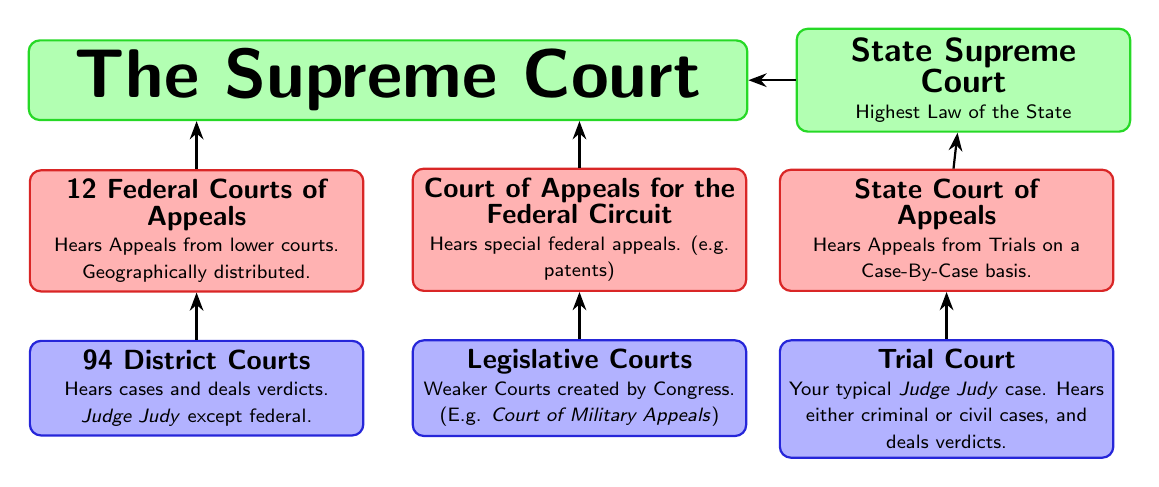
\begin{tikzpicture}[node distance = 6mm,
    box/.style = {rectangle, rounded corners, thick,
                    draw=#1!70!gray, fill=#1!30,
                    text width=4cm, minimum height=1cm, align=flush center,
                    font=\sffamily\linespread{.8}\selectfont}]
    % first row, on the bottom
    \node (94-district)     [box=blue]
    {\textbf{94 District Courts}\\
        \scriptsize
        Hears cases and deals verdicts. \textit{Judge Judy} except federal.};
    \node (legis-courts)    [box=blue, right=of 94-district]
    {\textbf{Legislative Courts}\\
        \scriptsize
        Weaker Courts created by Congress. (E.g. \textit{Court of Military Appeals})};
    \node (trial-court)     [box=blue, below right=0mm and 4mm of legis-courts.north east]
    {\textbf{Trial Court}\\
        \scriptsize
        Your typical \textit{Judge Judy} case. Hears either criminal or civil cases, and deals verdicts.};
    % second row
    \node (12-appeals)      [box=red, above=of 94-district]
    {\textbf{12 Federal Courts of Appeals}\\
        \scriptsize
        Hears Appeals from lower courts. Geographically distributed.};
    \node (court-appeals)   [box=red, above=of legis-courts]
    {\textbf{Court of Appeals for the Federal Circuit}\\
        \scriptsize
        Hears special federal appeals. (e.g. patents)};
    \node (state-appeals)   [box=red, above=of trial-court]
    {\textbf{State Court of\\ Appeals}\\
        \scriptsize
        Hears Appeals from Trials on a Case-By-Case basis.};
    % third row
    % firs calculate spreme court node width
    \path   let \p1 = ($(12-appeals.west)-(court-appeals.east)$),
                \n1 = {veclen(\x1,\y1)} in
            node (scotus)
                [box=green, font=\sffamily\Huge\bfseries,
                text width=\n1-2*\pgfkeysvalueof{/pgf/inner xsep},
                above=of $(12-appeals.north)!0.5!(court-appeals.north)$]
                {The Supreme Court};
    \node (state)       [box=green, right = of scotus]
    {\large\textbf{State Supreme Court}\\
        \scriptsize
        Highest Law of the State};
    \draw [-Stealth, thick]
        (trial-court)   edge (state-appeals)
        (state-appeals) edge (state)
        (state)         edge (scotus)
        (legis-courts)  edge (court-appeals)
        (court-appeals) edge (scotus.south -| court-appeals)
        (94-district)   edge (12-appeals)
        (12-appeals)     to  (12-appeals |- scotus.south) ;

\end{tikzpicture}
\end{document}